\documentclass[border=10pt]{standalone}
\usepackage{tikz}\usepackage{amsmath}\usetikzlibrary{arrows.meta}
\begin{document}
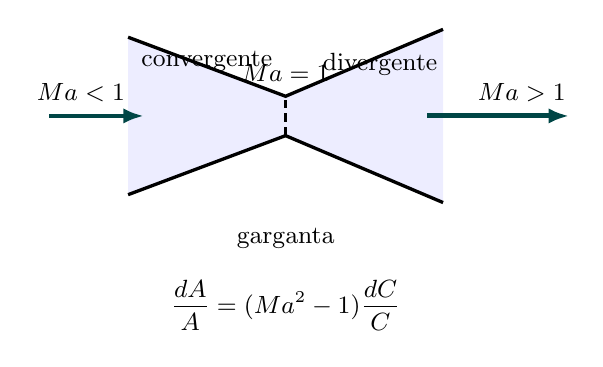
\begin{tikzpicture}[line width=1pt,>={Latex[length=2.6mm]}]
  % tobera convergente-divergente (de Laval)
  \fill[blue!7] (0,2)--(2,1.25)--(4,2.1) -- (4,-0.1)--(2,0.75)--(0,0)--cycle;
  \draw[line width=1.2pt] (0,2)--(2,1.25)--(4,2.1);
  \draw[line width=1.2pt] (0,0)--(2,0.75)--(4,-0.1);
  % garganta
  \draw[densely dashed] (2,0.75)--(2,1.25);
  \node[above] at (2,1.3){\small $Ma=1$};
  \node at (2,-0.55){\small garganta};
  % entrada subsonica (flecha corta)
  \draw[->,teal!55!black,line width=1.5pt] (-1.0,1.0)--(0.2,1.0);
  \node[above] at (-0.6,1.05){\small $Ma<1$};
  % salida supersonica (flecha larga)
  \draw[->,teal!55!black,line width=1.8pt] (3.8,1.0)--(5.6,1.0);
  \node[above] at (5.0,1.05){\small $Ma>1$};
  \node at (1.0,1.7){\small convergente}; \node at (3.2,1.65){\small divergente};
  \node at (2,-1.4){\small $\dfrac{dA}{A}=(Ma^2-1)\dfrac{dC}{C}$};
\end{tikzpicture}
\end{document}
